% Template for PLoS
% Version 1.0 January 2009
%
% To compile to pdf, run:
% latex plos.template
% bibtex plos.template
% latex plos.template
% latex plos.template
% dvipdf plos.template

\documentclass[10pt]{article}

% amsmath package, useful for mathematical formulas
\usepackage{amsmath}
% amssymb package, useful for mathematical symbols
\usepackage{amssymb}

% graphicx package, useful for including eps and pdf graphics
% include graphics with the command \includegraphics
\usepackage{graphicx}
\usepackage{wrapfig}
% cite package, to clean up citations in the main text. Do not remove.
\usepackage{cite}

\usepackage{color} 

% Use doublespacing - comment out for single spacing
%\usepackage{setspace} 
%\doublespacing


% Text layout
\topmargin 0.0cm
\oddsidemargin 0.5cm
\evensidemargin 0.5cm
\textwidth 16cm 
\textheight 21cm

% Bold the 'Figure #' in the caption and separate it with a period
% Captions will be left justified
\usepackage[labelfont=bf,labelsep=period,justification=raggedright]{caption}

% Use the PLoS provided bibtex style
\bibliographystyle{plos2009}

% Remove brackets from numbering in List of References
\makeatletter
\renewcommand{\@biblabel}[1]{\quad#1.}
\makeatother


% Leave date blank
\date{}

\pagestyle{myheadings}
%% ** EDIT HERE **


%% ** EDIT HERE **
%% PLEASE INCLUDE ALL MACROS BELOW

%% END MACROS SECTION

\begin{document}

% Title must be 150 characters or less
\begin{flushleft}
{\Large
\textbf{Final project: using competitive population firing rate models to describe buildup with ambiguous stimuli}
}
% Insert Author names, affiliations and corresponding author email.
\\
Sara Steele
\end{flushleft}

\section*{Introduction}
For some stimuli in the visual and auditory modalities with ambiguous grouping cues, there is a tendency for the likelihood of perceptual "splitting" to increase with time. For instance, with ambiguous moving plaids constructed from moving square wave gratings at intermediate speed and angle, observers have consistently reported first experiencing motion coherence, even when steady-state perception is biased towards transparent motion of the individual gratings \cite{Rubin2004}. Analogously, for ambiguous tone sequences in which observers report alternations between hearing grouped triplet patterns and split streams \cite{Noorden1975} (see Figure \ref{fig:percepts_timecourse}), there can be an initial period of buildup over which the probability of stream segregation increases. 


\begin{figure}[scale = 0.5]
	\centering
	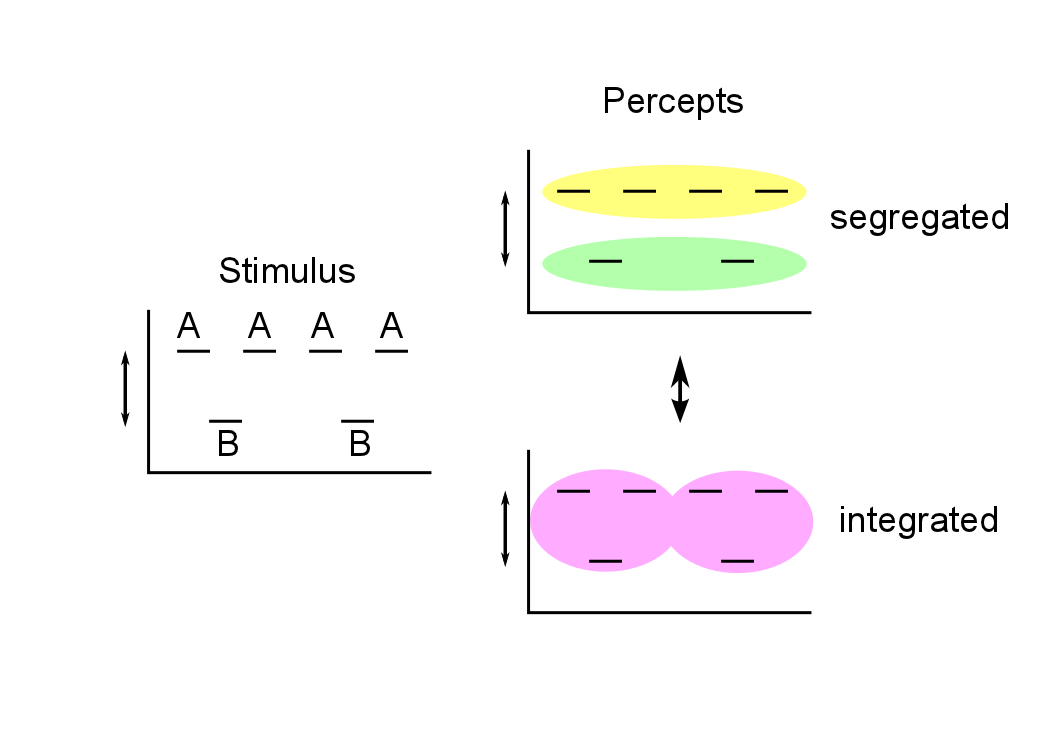
\includegraphics[scale=0.35]{../aba_stimulus-percepts}
	
\includegraphics[scale=0.47]{../percepts_timecourse}
	\caption{}
	\label{fig:percepts_timecourse}
\end{figure}


Indeed, the process of constructing buildup curves reflects the averaging over many trials of binary timecourses \ref{fig:TrialAvg}. I believe that the observation that the starting state is fixed is sufficient to account for transient increase in probability of split percepts, but that buildup is primarily a consequence of stochastic alternations between two states.

\begin{figure}
	\centering
	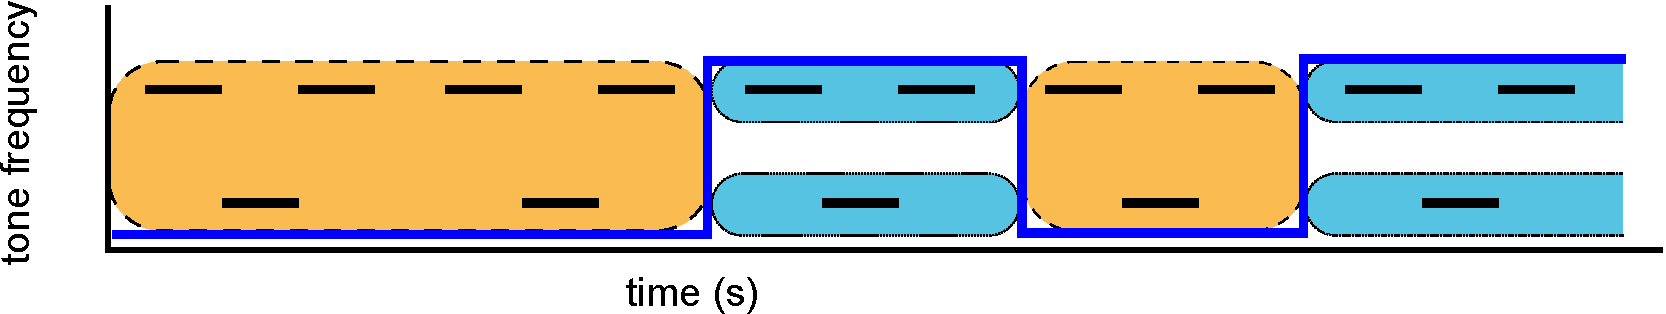
\includegraphics[scale=0.35]{../percepts_timecourse_binary}
	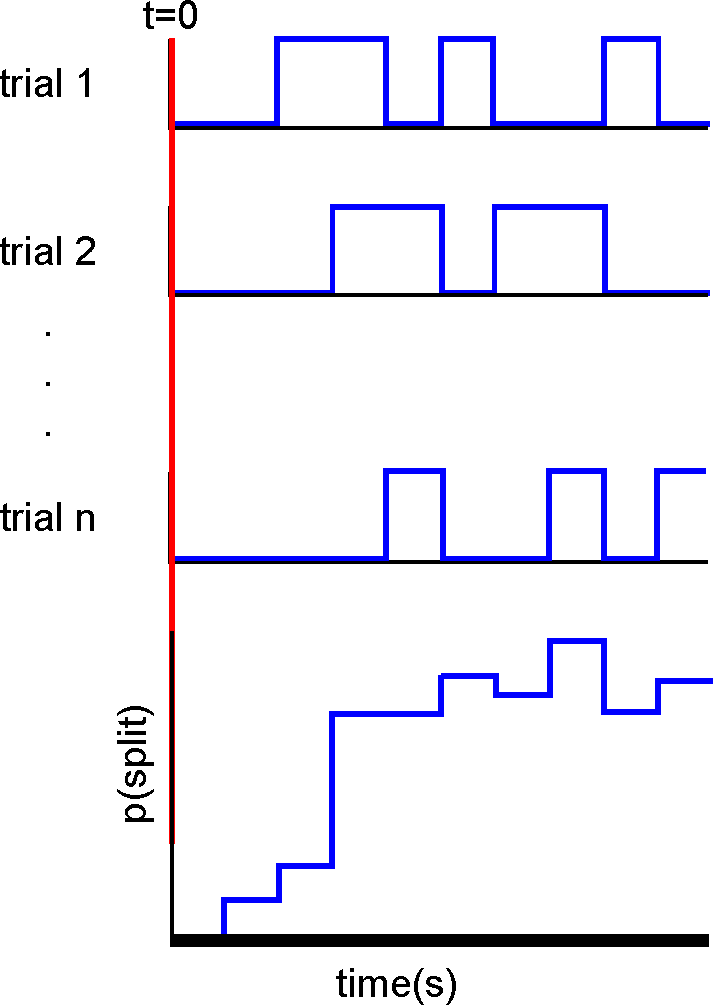
\includegraphics[scale=0.5]{../TrialAvg}
	\caption{}
	\label{fig:TrialAvg}
\end{figure}

I tested whether perceptual bistability models were capable of producing buildup if the starting state was fixed, and under which dynamical regimes.
\cite{Shpiro2009}

\section*{Methods}
\subsection*{Competition model simulations}
Competition model simulations followed the procedures reported previously in \cite{Shpiro2009} for population firing rate model with spike frequency adaptation. Specifically,

\begin{equation*}
	\begin{cases}
	\dot{u}_1 & = -u_1 +  f(-\beta u_2 - \gamma a_1 + I_1 + n_1) \\
	\tau_a \dot{a}_1 & = -a_1 + u_1\\
	\dot{n}_1 & = \frac{-n_1}{\tau_n} + \sigma \sqrt{\frac{2}{\tau_n}} \eta(t)\\
	\dot{u}_2 & = -u_2 +  f(-\beta u_1 - \gamma a_2 + I_2 + n_2) \\
	\tau_a \dot{a}_2 & = -a_2 + u_2\\
	\dot{n}_2 & = \frac{-n_2}{\tau_n } + \sigma \sqrt{\frac{2}{\tau_n}} \eta(t)
	
	\end{cases}
\end{equation*}

The variable $u_1$ corresponding to the short-time averaged firing rate of the population representing the ``grouped" perceptual state, and $u_2$ the firing rate of the population representing the ``split" perceptual state. The variables $a_1$ and $a_2$ represent the spike-frequency adaptation. Parameter $\gamma$ controls the strength of the adaptation, and $\beta$ controls the strength of suppression from the competing population. $I_1$ and $I_2$ are the external inputs driving the two populations, and $n_1$ and $n_2$ are independent Ornstein-Uhlenback noise generators with mean zero and variance $\sigma$, and a timescale of $\tau_n$. 
The input-output function used was a sigmoid, with $f (x) = 1/(1 + exp(−(x − \theta )/ k))$. 

The simulation was carried out on a characteristic neuronal timescale, with one unit of time corresponding to 10 msec. The following parameter values are used: $k = 0.1, \theta = 0, \beta = 1$. Time constants given in simulation time units were $\tau_a = 200, \tau_n = 10$. The values of the external inputs to the populations $I_1$ and $I_2$, the adaptation gain $\gamma$ and the noise strength $\sigma$ were varied as specified in the text, with the value of $\sigma$ scaled in relation to the integration time step by $1/\sqrt{dt}$ to keep specified variance per unit time. Simulations were implemented in MATLAB using forward Euler integration with a time step of 0.1 (1 msec real time).

For each combination of parameter values, I simulated 500 trials of length 10 s with initial conditions $u_2(0), a_1(0), a_2(0), n_1(0), n_2(0) = 0$ and $u_1(0) = 0.5$; thus, at the beginning of each simulated trial, the first population to become dominant was always that corresonding to the first percept. With the resulting population firing rate timecourses, I obtained dominance durations by finding time points of the zero crossings of the differences of the firing rates. Using the samples of dominance durations obtained for each population (over 1000 durations for each population with each parameter set), I fitted gamma densities using maximum likelihood estimation. Simulated experimental buildup curves were constructed by averaging across trials the binary timecourse $u_2 > u_1$. 


% Results and Discussion can be combined.
\section*{Results}
\subsection*{Buildup curves look most realistic for noise-driven, not adaptation driven, alternation regimes}
See Figure \ref{fig:mono_vs_periodic}. Noise driven switching is necessary for buildup functions that look like those presented in the literature; however, in principle the apparent monotonically increasing likelihood of split percepts over time could also be accomplished by averaging together the timecourses of multiple oscillators with different periods. However, there have been no reports whatsoever of oscillatory buildup functions.

\begin{figure}[scale = 0.8]
   \begin{center}
   
   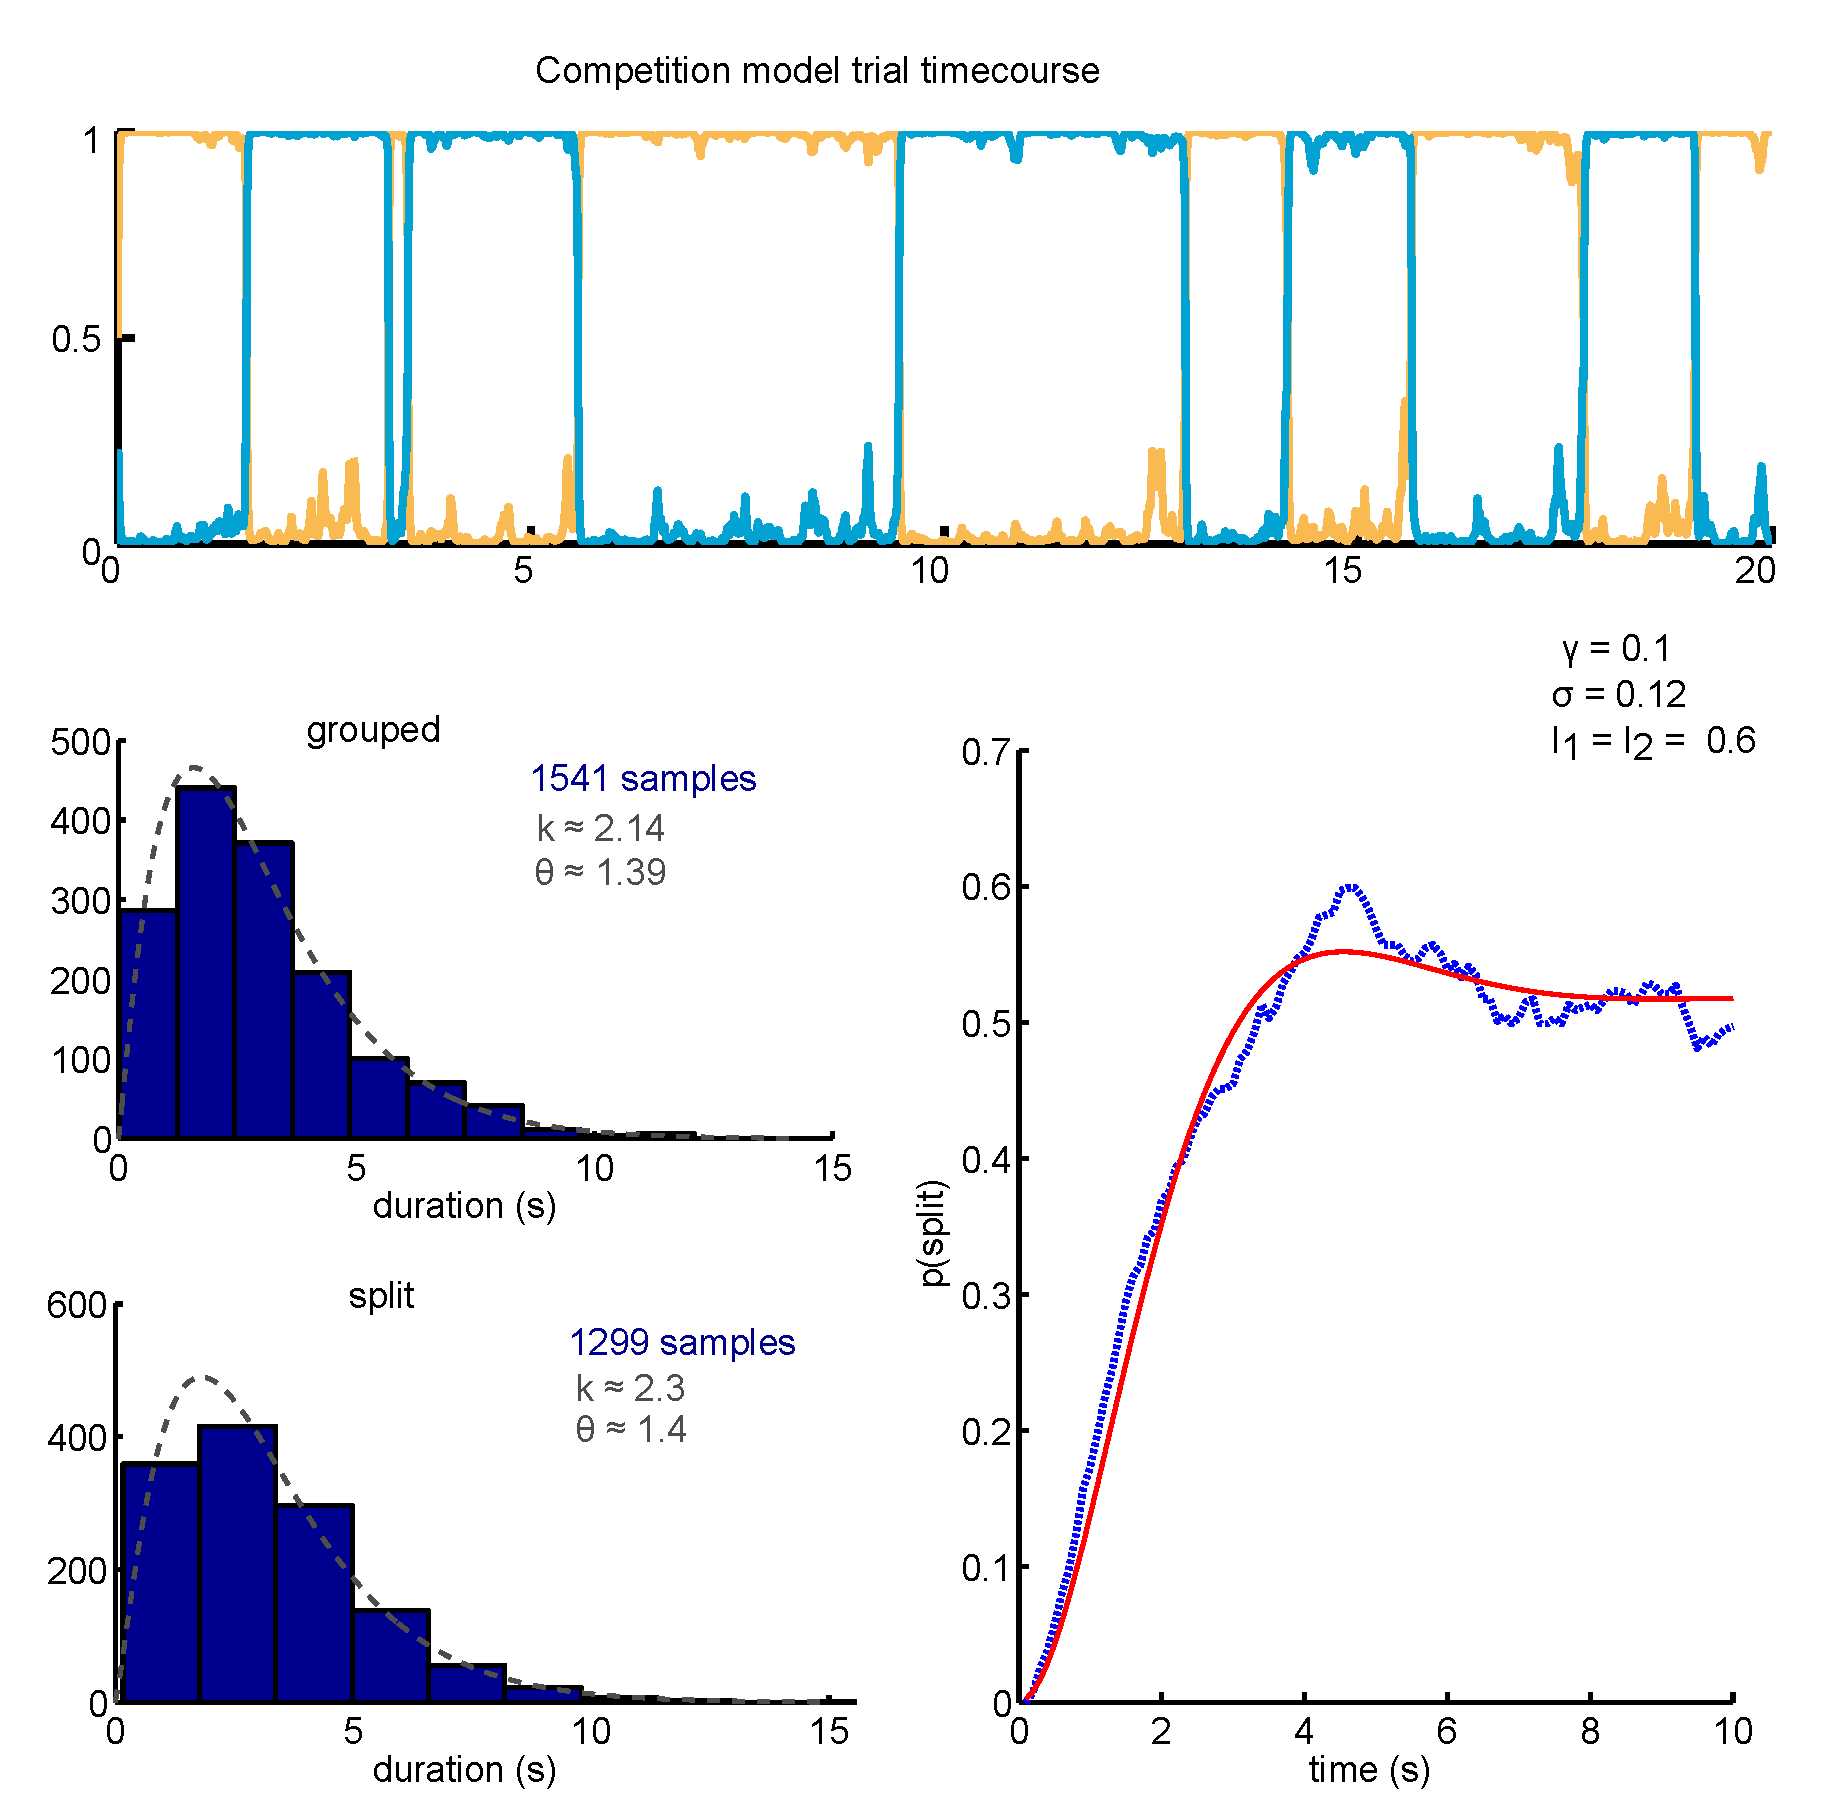
\includegraphics[scale=0.33]{BUFs_hists_lowadapt}
   
   \includegraphics[scale=.33]{hi_adapt_low_noise_equal_inputBUFshists}      
   \caption{Buildup functions for low-adaptation and high-adaptation, low noise parameter regimes.}
   	\label{fig:mono_vs_periodic}
   \end{center}
\end{figure}


\begin{figure}[scale = 0.4]
   \begin{center}
   	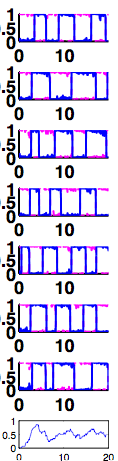
\includegraphics[scale = 0.5]{../clocky_switches} % requires the graphicx package
   \caption{When switches are driven by adaptation, the system behaves as a noisy oscillator around a fixed period. Because of the "clockiness" of the timecourses, the oscillations appear in the average.}
   	\label{fig:example}
   \end{center}
\end{figure}




\subsection*{Buildup occurs faster for less ambiguous stimuli}

The time it takes to achieve the steady state fractional dominance ratio should depend on both how far the original fractional dominance ratio from the steady state as well as the strength of the biasing input in favor of either of the two states. In \ref{fig:ambiguous_vs_biased} we see that the strength of the biasing input is much more important to defining the overall timescale of buildup than the distance between starting and steady states. This effect is in contrast to the effect on mean durations; mean durations for grouped percepts in the ambiguous case was 8.07 s, and for split 7.57 (grand mean =  7.8) whereas for the biased case, the average grouped duration was 1.29 s, the averaged split duration was 18.213, and the grand mean was 9.75. So while switches occurred more frequently in the ambiguous case, the time to half-maximum was also longer.

\begin{figure}[scale=0.5]
   \begin{center}
   
   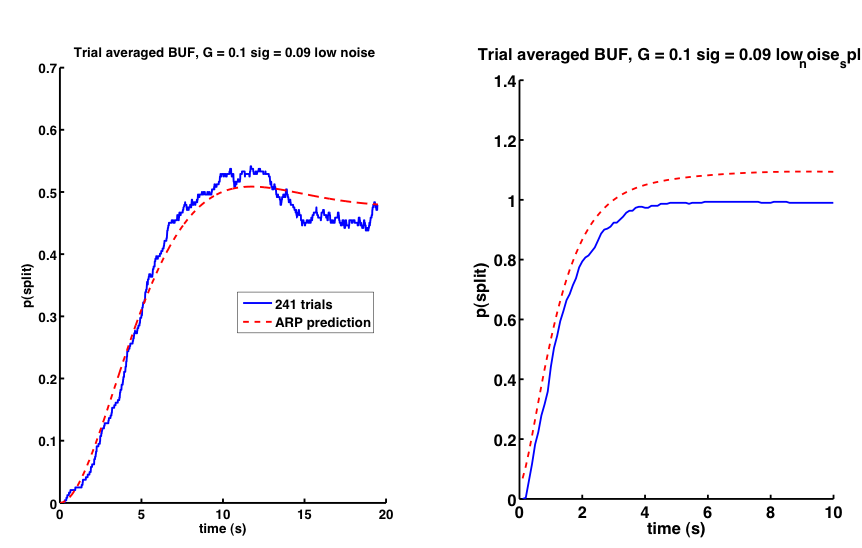
\includegraphics[scale=0.33]{../ambiguous_vs_biased}
   
   \caption{When stimulus is very ambiguous, leading to steady state equal fractional dominance durations, buildup is slow-- left, half-maximum is achieved after about 5 s. However when the stimulus is strongly biased, the steady state is achieved in much shorter time (~2s), even when this is further from the starting state.}
   	\label{fig:ambiguous_vs_biased}
   \end{center}
\end{figure}
%
\section*{Discussion}

These results support the growing body of research suggesting that accumulation of adaptation is not the primary cause of alternations \cite{Pastukhov2013}. An oscillator regime would produce extremely oscillatory buildup functions unless the buildup function reflected the average of many different oscillators with different periods or phases. To my knowledge this is the first time that buildup has been produced through model simulations of this kind, and the most parsimonious explanation for the results we see is that the alternations experienced by observers during these kinds of ambiguous stimuli are driven by noise, not adaptation.

%(BUT ARE THERE EXPERIMENTS IN WHICH BUILDUP IS OBSERVED FOR SOME NON-AMBIGUOUS STIMULUS? DOES BUILDUP EXIST FOR NON ABA STIMULI, BECAUSE THAT'S WHY IT'S APPEALING AND ANY STIMULUS THAT SHOWS BUILDUP MIGHT BE USEFUL FOR ALTERNATION)

% You may title this section "Methods" or "Models". 
% "Models" is not a valid title for PLoS ONE authors. However, PLoS ONE
% authors may use "Analysis" 


% Do NOT remove this, even if you are not including acknowledgments
\section*{Acknowledgments}


\section*{References}
% The bibtex filename
\bibliography{/Users/steeles/Documents/library}


\end{document}
